% Paper 003 manuscript, v1.0.
%
% Content source: paper003_manuscript_negative_v1.0.md, which stays authoritative.
% Figures: paper003_manuscript_negative_v1.0.md's figures/ directory, expected at
% ./figures/ beside this file (the Overleaf zip is packed that way).
%
% BEFORE SUBMISSION, two things:
%   1. Verify every entry in paper003_references_v1.0.bib. The volume numbers,
%      page ranges and years have not been checked against published records, and
%      two references named in the positioning document are deliberately absent.
%   2. Set \draftnotefalse below to remove the verification banner.
\documentclass[10pt]{article}
\usepackage[a4paper,margin=25mm]{geometry}
\usepackage[T1]{fontenc}
\usepackage[utf8]{inputenc}
\usepackage{amsmath,amssymb}
\usepackage{graphicx}
\usepackage{booktabs,tabularx,array}
\usepackage{enumitem}
\usepackage{caption}
\usepackage[numbers,sort&compress]{natbib}
\usepackage{xurl}
\usepackage[colorlinks=true,allcolors=blue]{hyperref}
\setlength{\parindent}{0pt}
\setlength{\parskip}{0.55em}
\renewcommand{\arraystretch}{1.12}
\graphicspath{{figures/}}

\newif\ifdraftnote
\draftnotetrue   % <- set to \draftnotefalse before submission

\title{What a Missing-Relation Cell Requires:\\Four Candidate Relations and a Negative Result Under Physical Contact}
\author{Seonhye Gu\thanks{This work was independently conducted by the author as personal research while affiliated with the AI-Based Surgical Robot Innovation Lab. The affiliation is provided for identification purposes only and does not imply official laboratory output, institutional endorsement, or sponsorship.}\\
\small AI-Based Surgical Robot Innovation Lab}
\date{}

\begin{document}
\maketitle

\ifdraftnote
\begin{center}
\fbox{\parbox{0.92\textwidth}{\small\textbf{Draft note, not for submission.} The
bibliography has not been verified against published records. No confirmatory run
was performed: all physical evidence is calibration, and the preregistration
excludes calibration from confirmatory estimates. Section~\ref{sec:notclaimed}
states precisely which claims this record does and does not support. Remove this
box by setting \texttt{\textbackslash draftnotefalse}.}}
\end{center}
\fi

\begin{abstract}
Prior work in this program showed that structured failure after parameter repair
can justify a prepared increase in target-model \emph{order}---a missing dynamic
mode. The natural next cell in the taxonomy is a missing \emph{relation}: a
residual conditioned not on an unrepresented state variable of the target, but on
a second entity. We preregistered a design for that cell, built it, and report a
negative result.

We evaluated four candidate relations against three requirements fixed in
advance: the relation's effect must exceed the task tolerance, a single-entity
model of the target must not suffice, and the relation must not be reducible to a
dynamic mode. \textbf{Collision} fails the first---a struck target's displacement
per contact is of the order of the interaction radius, five independent
measurements placing it below the 20~mm placement criterion. \textbf{Carriage}
fails the second---a model observing only the target's own trajectory matched the
relational arm exactly. \textbf{Capture}---a body arrives at a still target and
carries it off---satisfies all three under injected coupling, where the
relational arm scores 0.650 against a single-entity competitor's 0.000 across 200
preregistered paired cells (one-sided exact McNemar, 130 discordant pairs, none
the competitor's, \(p = 7.3 \times 10^{-40}\)).

Under \textbf{physical contact} in Isaac Sim it fails the third. Across 107 cells
and three configurations of a surgical needle driver, the constant-velocity mode
operator lands \textbf{0.957 to 1.000} of cells while the relational arm lands
0.174 to 0.583 and \textbf{never wins a paired cell that the single-entity arm
loses} (0 against 4, twice). The relation is made necessary by
\emph{intermittency}, and the arm requires a median of 22 steps to come to rest
after its goal stops, against a commanded pause of 4 and 54 steps of grip on the
object: the pause never begins.

The contribution is the requirement set, the measurement that each candidate
fails, and a physical criterion recovered by sweeping the carrier's settling time
under injected coupling: the mode operator returns once settling reaches the
carrier's duty-cycle period, 0.133 to 0.917 across that threshold. The same sweep
refutes the tidier account we started with---the relational arm does \emph{not}
collapse under a smoothed carrier, so settling explains the mode operator's
return and not the relational arm's physical failure, which remains open.

\textbf{Keywords:} world models, structural adaptation, relational models,
negative results, preregistration, embodied control, surgical simulation
\end{abstract}

\section{Introduction}

An embodied agent whose predictions fail can respond at three depths. It can
repair parameters inside a fixed model class. It can expand the class to
represent a state variable it lacked---\emph{model-order expansion}. Or it can
expand the class to represent a \emph{dependence on another entity}, which is a
change of a different kind: the model gains not a variable but an argument.

This paper concerns the third. The program's governing principle is that
intelligence chooses the \emph{smallest sufficient change}, so a relational
expansion is warranted only where a mode expansion is insufficient. That is a
demanding condition, and this paper's result is that it is more demanding than it
appears.

Relational and object-centric dynamics models establish \emph{how} such structure
is represented \citep{battaglia2016interaction,kipf2018nri,kipf2020cswm}. This
paper does not compete on that axis: it assumes a prepared relation-module
operator and asks \emph{when} such an operator becomes necessary. Classical
model-order selection asks the analogous question one level down
\citep{ljung1999system}.

We report a negative result and a positive characterisation. The negative result
is that the task family we built does not exhibit a missing relation under
physical contact: the mode operator suffices. The positive characterisation is
the requirement set that makes the negative result informative---three task-level
requirements, each of which eliminated a candidate relation on measured grounds,
and one physical requirement on the manipulator that emerged from the failure.

\subsection{Why publish this}

Three reasons, in ascending order of importance.

\begin{enumerate}[leftmargin=*]
\item The requirement set is reusable. Anyone building a missing-relation
benchmark must satisfy it, and three of the four requirements are cheap to check
before any hardware is involved.
\item The mode/relation boundary is not where the taxonomy places it. A
constant-velocity operator absorbed a coupling designed specifically to be
outside it. That is a finding about the taxonomy, not about this scene.
\item The failure is a \emph{shortcut}, not a null
\citep{geirhos2020shortcut}. The relational task was solvable---the oracle arm
lands 1.000 of physical cells---by a mechanism simpler than the one the benchmark
names, and that mechanism was named in advance as the discriminating control.
\end{enumerate}

\section{Design, locked before measurement}

The design was locked before any physical cell was run, and no locked rule was
changed afterwards.

\subsection{Task}

A commitment point. The agent commits to an irreversible placement onto a target
that a reference body captures and carries. The action takes
\texttt{dispense\_latency} steps and lands wherever the target is at completion;
there is no correction. The structure is required, not incidental---a continuous
reach-and-hold version produced no separation between any arms, because
continuous re-aiming averages prediction error away.

Placement tolerance \textbf{20~mm}, on two grounds fixed before this study
existed: the task family's own termination threshold, and the block's
half-height.

\subsection{Arms}

\begin{center}
\begin{tabular}{@{}lll@{}}
\toprule
Arm & Target model & Role \\
\midrule
A & Frozen & Secondary baseline \\
B & Parameter repair, independent-entity model & Primary comparator \\
\textbf{C} & \textbf{Mode expansion---the prepared operator} & \textbf{Discriminating control} \\
\textbf{SELF} & \textbf{The target's own trajectory only} & \textbf{Decisive competitor} \\
D & Relation expansion & Primary intervention \\
D\(^{*}\) & Relation with the true landing supplied & Diagnostic ceiling \\
\bottomrule
\end{tabular}
\end{center}

All arms share controller, task, tolerance and commit policy, and differ only in
the predicted landing point. Arm~D falls back to arm~B when its gate does not
fire, so \(D \geq B\) holds by construction; the informative quantities are how
often D engages and how much it wins by when it does, and both are reported
throughout.

SELF is deliberately \textbf{ungated}---arm~D may act only when the
relation-adequacy gate fires, SELF acts whenever its own pattern is identifiable.
The asymmetry favours the competitor by design.

\subsection{Requirements on the relation, fixed in advance}
\label{sec:requirements}

\begin{itemize}[leftmargin=*]
\item \textbf{R1---the effect must exceed the tolerance.} The relation must move
the target further than the task's own success criterion, or no arm can be
distinguished by it.
\item \textbf{R2---the relation must be necessary.} A model observing only the
target's own trajectory must not suffice. This is what arm SELF tests.
\item \textbf{R3---the relation must not reduce to a mode.} The second entity's
influence must not be expressible as a dynamic mode of the target alone. This is
what arm~C tests.
\item \textbf{R4---onset must be observable, or the claim must be scoped after
onset.}
\end{itemize}

R4 was settled early and negatively, and the paper's claim is scoped accordingly:
in the control worlds a body approaches the target and nothing happens, and it
approaches \emph{closer} than in the treatment---12 and 14~mm against 42~mm, in
1.00 of cells. Up to the moment of contact a capturing approach and a
non-capturing one are the same observation, so no arm could predict onset and the
paper does not claim to.

\section{Four candidates, and where each fails}

\begin{center}
\begin{tabular}{@{}lccc@{}}
\toprule
Relation & R1 effect \(>\) tol. & R2 necessary & R3 not a mode \\
\midrule
Collision---struck and released & \textbf{no} & yes & yes \\
Carriage---rides throughout & yes & \textbf{no} & --- \\
Capture, injected coupling & yes & yes & yes \\
\textbf{Capture, physical contact} & yes & \textbf{no} & \textbf{no} \\
\bottomrule
\end{tabular}
\end{center}

\subsection{Collision fails R1}

The push moves the target away, which reduces penetration, which reduces the
push. Displacement per contact therefore settles at the order of the interaction
radius, below the 20~mm criterion. Measured five independent ways. This is a
structural property of a penetration-driven contact law, not a tuning failure:
raising the body's speed raises the equilibrium separation, not the displacement.

\subsection{Carriage fails R2}

A target that rides its reference throughout clears the tolerance easily and
makes the relation unnecessary---a single-entity model of the target's own
trajectory matched the relational arm \textbf{exactly}, cell for cell. The second
entity supplies nothing the target's own history does not.

\subsection{Capture satisfies all three under injected coupling}

Capture---a body arrives at a \emph{still} target and carries it off---was
designed against both failures. Before the arrival the target is perfectly still,
so its own history says nothing; afterwards it rides, so the effect accumulates
without bound. It carries a third property that R2 turns on: the carrier moves
\textbf{intermittently}, and the pauses are not predictable from the target
alone.

\textbf{R2, preregistered.} The rule was fixed in writing before the SELF arm was
implemented. On 200 paired cells at offsets [+4, +6], arm~D scored \textbf{0.650
against SELF's 0.000}---130 discordant pairs, \textbf{none of them the
competitor's}, one-sided exact McNemar \(p = 7.3 \times 10^{-40}\). On the
amended band [+4, +8] with fresh seeds, 0.735 against 0.045 and a discordant
split of \textbf{146 to 8}.

\textbf{All four arms on one run}, which the two statements above deliberately
are not---a preregistered pairwise comparison scores two arms, and reading a
four-arm table off two runs with different seeds and different commit bands is
how a figure in this project first went wrong:

\begin{center}
\begin{tabular}{@{}lrrrr@{}}
\toprule
CPU, injected, 60 cells & arm B & arm C & SELF & \textbf{arm D} \\
\midrule
& 0.000 & 0.133 & 0.083 & \textbf{0.417} \\
\bottomrule
\end{tabular}
\end{center}

\textbf{R1 and R3 hold here.} Arm~B lands nothing, so the effect exceeds the
tolerance; arm~C lands 0.133, so the mode operator helps only partially, which is
exactly the partial help the design requires and does not get under contact.

The competitor was not broken. It acted on 0.675 of cells, and its median miss
\emph{when acting} was 60.0~mm against 30.0~mm when it declined---it extrapolates
through a pause it cannot see, which is exactly the information the relation
supplies.

\textbf{Two limits were measured with it, and both are reported rather than
relied on.} The single-entity arm catches up from commit offset \textbf{+30}, a
little over two burst cycles after the arrival; the protocol's commit window is
[\(-6\), +6], where SELF scores \(\leq 0.02\). And what stops arm~D first is its
own gate rather than the competitor---the constant-velocity statistic climbs as
the carry lengthens, and arm~D declines exactly where it crosses the ceiling
written to keep a drift control out.

\subsection{Capture fails R2 and R3 under physical contact}

The Isaac Sim lift scene and its needle variant, a surgical needle driver, with
the same cell loop and the same arms. The simulator replaces the arithmetic: the
cell commands the bodies, steps physics, and \emph{reads} where the object went.

The scene produces the relation. \textbf{60 of 60 cells were captures} by the
preregistered verdict, so the outcome the calibration pilot was written to
catch---``the scene does not produce a capture at all''---did not occur.

\begin{figure}[ht]
\centering
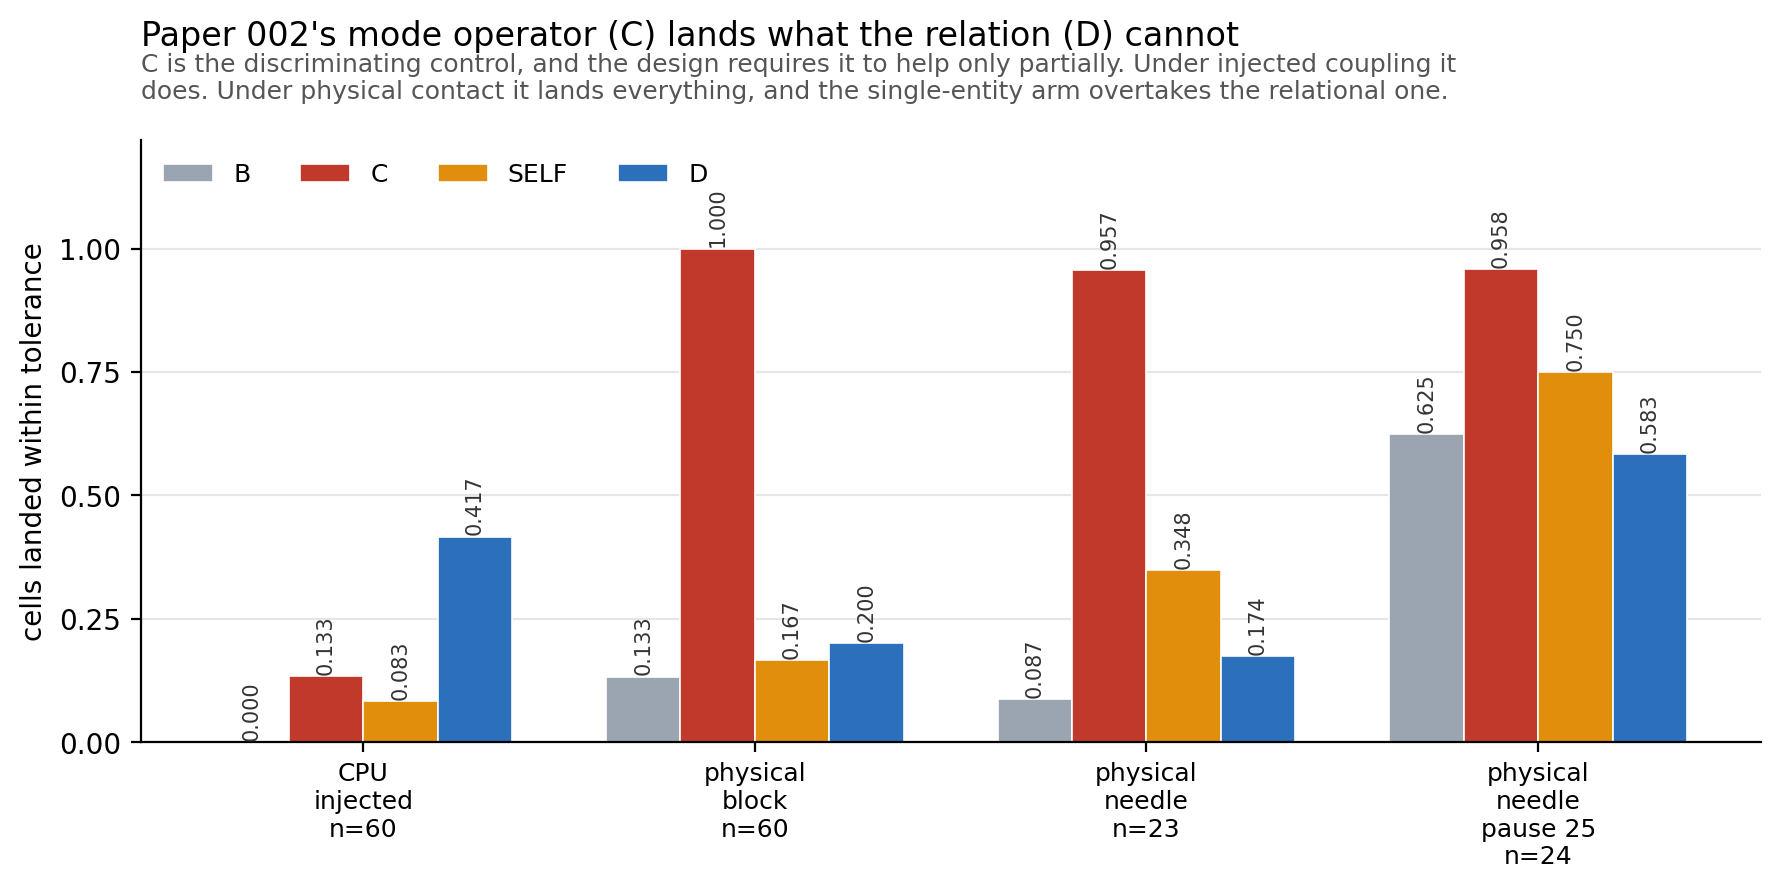
\includegraphics[width=\textwidth]{fig2_arm_scores.png}
\caption{Every arm, injected coupling and three physical configurations. Arm~C is
the discriminating control, and the design requires it to help only partially.
Under injected coupling it does. Under physical contact it lands everything.}
\label{fig:arms}
\end{figure}

\begin{center}
\begin{tabular}{@{}lrrrrrrr@{}}
\toprule
Configuration & A & B & \textbf{C} & SELF & \textbf{D} & D\(^{*}\) & cells \\
\midrule
block & 0.000 & 0.133 & \textbf{1.000} & 0.167 & \textbf{0.200} & 1.000 & 60 \\
needle, pause 4 & --- & 0.087 & \textbf{0.957} & 0.348 & \textbf{0.174} & --- & 23 \\
needle, pause 25 & --- & 0.625 & \textbf{0.958} & 0.750 & \textbf{0.583} & --- & 24 \\
\bottomrule
\end{tabular}
\end{center}

\textbf{R3 fails.} A constant-velocity model lands essentially every cell. The
design requires \(\mathrm{success}(D) - \mathrm{success}(C)\) to clear a positive
margin; the difference is negative in all three configurations, by between 0.37
and 0.80.

\textbf{R2 fails too, and in the competitor's favour.} Across the 47 needle
cells, \textbf{arm~D wins zero paired cells that SELF loses}, while SELF wins
four that arm~D loses---in each configuration separately. Under injected coupling
the same comparison ran 146 to 8 in arm~D's favour.

\begin{figure}[ht]
\centering
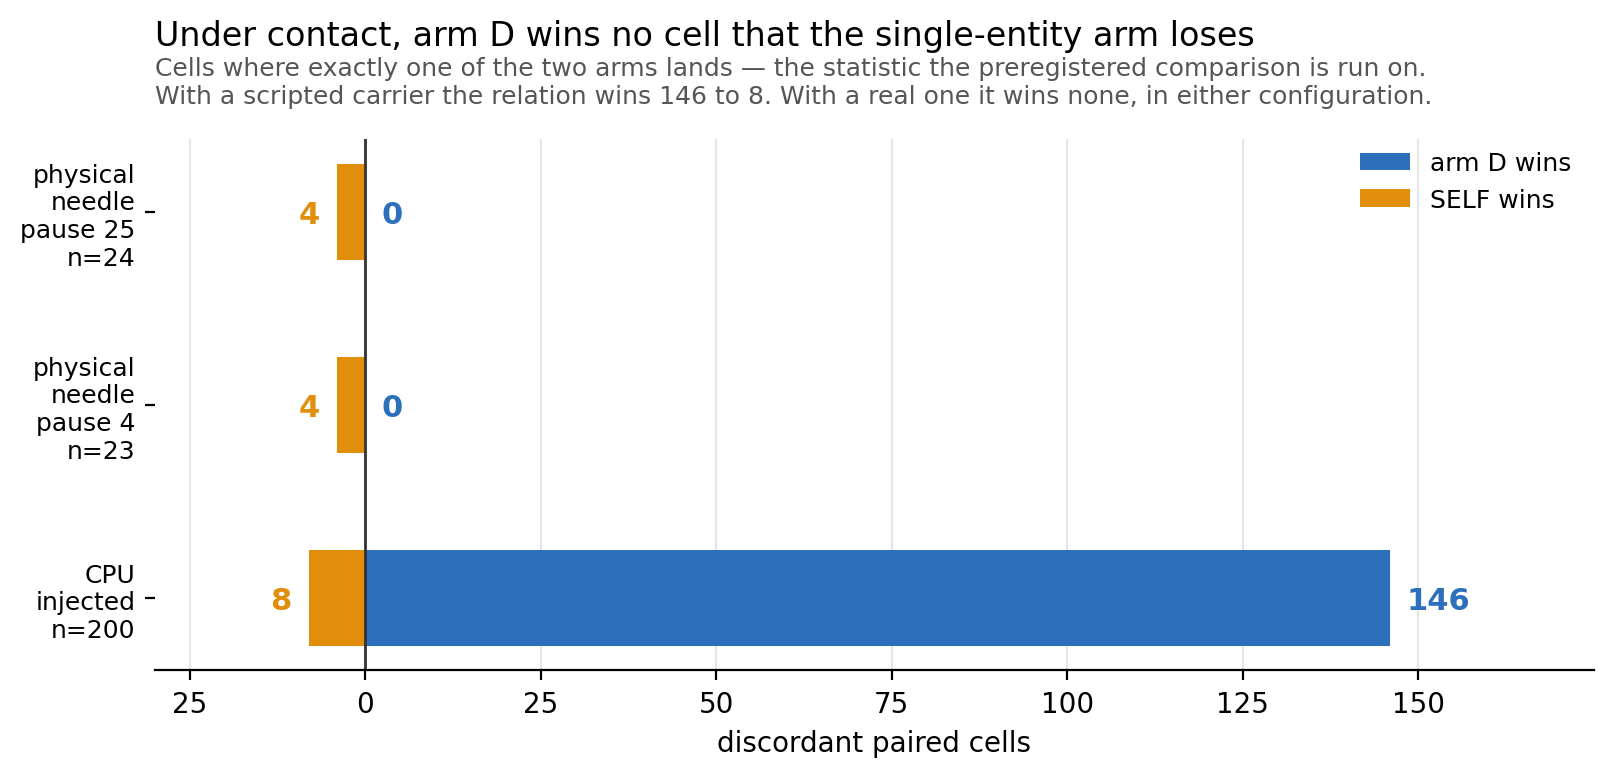
\includegraphics[width=\textwidth]{fig3_discordant_pairs.png}
\caption{Cells where exactly one of arm~D and SELF lands---the statistic the
preregistered comparison is run on. With a scripted carrier the relation wins 146
to 8. With a real one it wins none, in either configuration.}
\label{fig:discordant}
\end{figure}

\section{Why, as far as we can show it: the carrier cannot stop}

The relation is made necessary by \textbf{intermittency}. A target that rides
continuously moves at constant velocity, and then the mode operator suffices by
construction; the \emph{pauses} are what neither a single-entity nor a mode model
can represent. On CPU the carrier is a scripted point and the intermittency is
exact.

A real arm does not stop when told. Measured over 139 goal-pauses in 20 cells,
the arm takes a median of \textbf{22} steps to read as stopped after its goal
stands still, with a ninetieth percentile of 59 and a maximum of 85---against a
commanded pause of 4~steps. \textbf{The pause never begins.} What reaches the
object is not the commanded square wave but a heavily smoothed version of it,
quantified in Section~\ref{sec:sweep} as a velocity ripple of 0.174 against the
commanded 1.000, and a ride that smooth is precisely the case the mode operator
was built for.

\begin{figure}[ht]
\centering
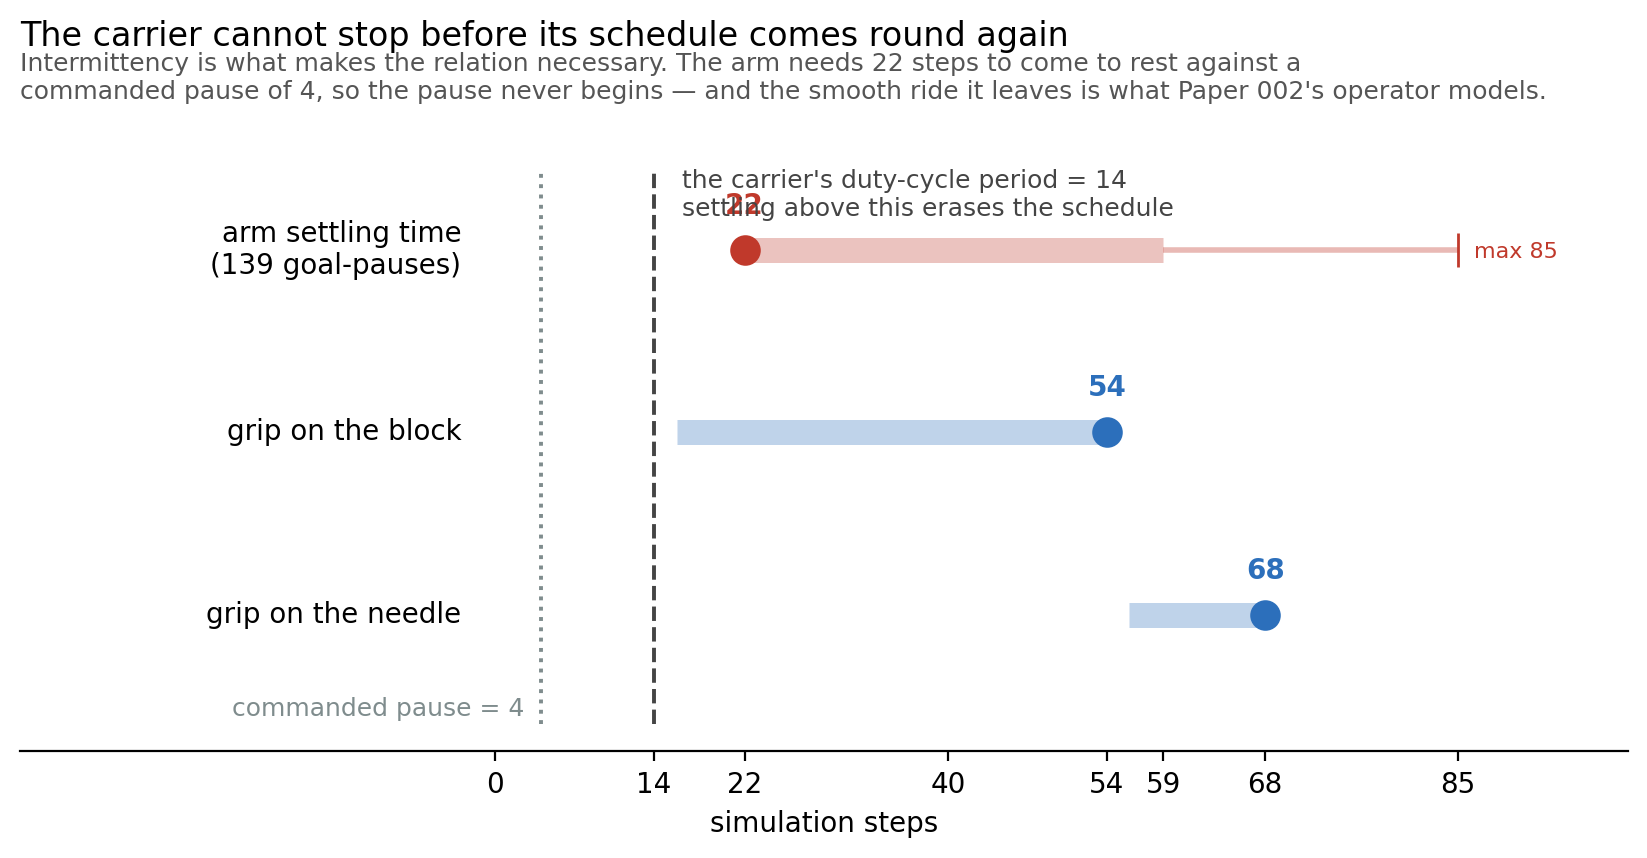
\includegraphics[width=\textwidth]{fig1_carrier_cannot_stop.png}
\caption{The arm's settling time against its grip duration and the carrier's
duty-cycle period. Intervals are the order statistics actually measured.}
\label{fig:mechanism}
\end{figure}

\subsection{Two repairs, derived in advance, both tried}

\textbf{A better-held object.} The manipulator is a needle driver and the block is
not what it was built to grip, so the needle is the favourable case: held 68
steps at the median against the block's 52 over the matched cells (54 over all
60), with a tenth percentile of 56 against 16. Arm~C: \textbf{0.957}. The mode
operator still lands everything, and on the needle the single-entity arm
overtakes the relational one.

\textbf{Restoring the pause.} The rule was written before the settling time was
measured: \emph{the pause must exceed the arm's settling time, plus the gate's
minimum ride so that the stillness is observable}---both quantities already
declared. That gives \textbf{25 steps} at the median. The needle's 68-step carry
has room for one such pause where the block's does not. Run at 25: arm~C moves
from \textbf{0.957 to 0.958}.

\subsection{The long-pause configuration does not cleanly test what it was built to test}
\label{sec:longpause}

\textbf{Arm~B rises from 0.087 to 0.625.} Arm~B is a zero-order aim and succeeds
when the target barely moves during the dispense. With 25 steps of pause in a
29-step cycle most of the carry is dead time, so most commit windows land where
nothing is happening and the trivial arm wins. Every arm rose except C, which had
nowhere to rise to.

This was written down as one of three possible readings \textbf{before} the run:
\emph{``C drops but B is also high \(\rightarrow\) the task setup is broken and
eligibility must exclude pause-window commits.''} Section~\ref{sec:unexplained}
confirms it on CPU---the same signature reproduces under injected coupling, so
this row's anomaly belongs to the commit policy and needs no explanation from the
physics.

It is reported as a limitation of that row rather than repaired, because
repairing it means changing the preregistered commit policy to exclude dispense
windows containing no target motion---a new design, not a fix to this one.
\textbf{The conclusion therefore rests on the two configurations where arm~B is
at 0.087 and 0.133}, cells genuinely hard for a zero-order model, and arm~C is at
0.957 and 1.000 anyway.

\subsection{The physical requirement, measured rather than asserted}
\label{sec:sweep}

An earlier draft of this section stated a criterion and derived it from two
physical measurements taken separately. That is an inference, not a result, so we
tested it. Settling time is a property of the \textbf{carrier}, and under
injected coupling the carrier is ours to specify: we added a settling parameter
that smooths the commanded velocity so the body coasts for exactly that many
steps past a stop, swept it over the configuration where the relation is known to
be necessary, and fixed four numbered predictions in writing before implementing
any of it.

\textbf{All four predictions failed.} What survives is better supported than what
was asserted, one claim is withdrawn outright, and one previously open question
is closed.

\begin{figure}[ht]
\centering
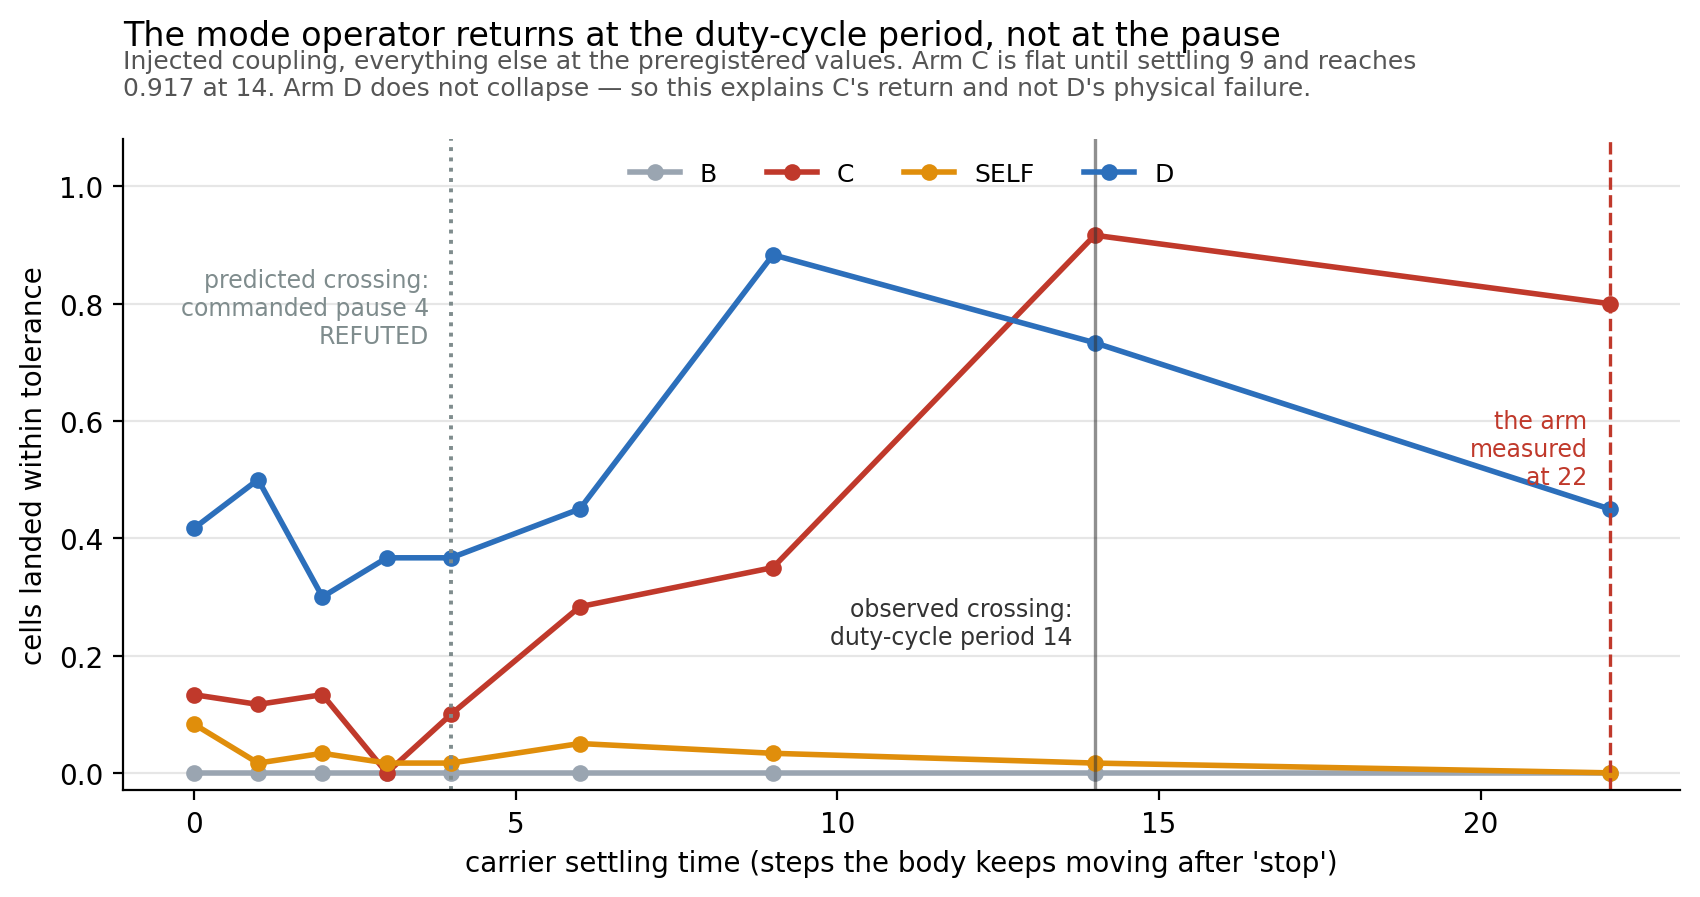
\includegraphics[width=\textwidth]{fig4_settling_sweep.png}
\caption{The predicted crossing, at the commanded pause, is marked and labelled
refuted. The observed crossing is at the duty-cycle period. Arm~D does not
collapse.}
\label{fig:sweep}
\end{figure}

\begin{center}
\begin{tabular}{@{}lrrrrr@{}}
\toprule
settling & B & C & SELF & D & D\,:\,SELF discordant \\
\midrule
0---the scripted point & 0.000 & 0.133 & 0.083 & 0.417 & 21\,:\,1 \\
4---the commanded pause & 0.000 & 0.100 & 0.017 & 0.367 & 21\,:\,0 \\
9---the commitment latency & 0.000 & 0.350 & 0.033 & 0.883 & 51\,:\,0 \\
\textbf{14---the schedule's period} & 0.000 & \textbf{0.917} & 0.017 & 0.733 & 43\,:\,0 \\
22---the arm's measured settling & 0.000 & \textbf{0.800} & 0.000 & 0.450 & 27\,:\,0 \\
\bottomrule
\end{tabular}
\end{center}

\textbf{The scale is the carrier's duty-cycle period, not its commanded pause.}
Arm~C does not move until settling reaches 9 and reaches 0.917 at \textbf{14},
which is the sum of the burst and pause durations. Smoothing does not eat the
pause from one end; it low-pass filters the whole waveform, and the intermittency
survives as a \textbf{ripple} in the carrier's velocity whose size falls as the
window approaches the period.

\textbf{The variable is that ripple, and arm~C tracks it at \(r = -0.940\).}

\begin{center}
\begin{tabular}{@{}lrrrrrr@{}}
\toprule
settling & 0 & 4 & 6 & 9 & 14 & 22 \\
\midrule
velocity ripple & 1.000 & 0.800 & 0.571 & 0.400 & 0.067 & 0.174 \\
arm C & 0.133 & 0.100 & 0.283 & 0.350 & \textbf{0.917} & \textbf{0.800} \\
\bottomrule
\end{tabular}
\end{center}

The ripple is not monotone in settling---a boxcar cancels a periodic signal
exactly only when its width is an integer multiple of the period---and arm~C is
not monotone either, scoring lower at settling 22 than at 14 for exactly that
reason. This was found by a unit test failing on a stronger claim, and it is why
we state the criterion on the ripple rather than on a threshold in settling.

\textbf{The criterion evaluated at matched ripple}, which puts CPU and physical
configurations on the same axis:

\begin{center}
\begin{tabular}{@{}lrrrr@{}}
\toprule
& period & settling & ripple & arm C \\
\midrule
CPU, scripted point & 14 & 0 & 1.000 & 0.133 \\
CPU & 14 & 22 & 0.174 & 0.800 \\
\textbf{physical, block} & 14 & 22 & 0.174 & \textbf{1.000} \\
CPU & 35 & 22 & 0.435 & 0.350 \\
\textbf{physical, needle, long pause} & 35 & 22 & 0.435 & \textbf{0.958} \\
\bottomrule
\end{tabular}
\end{center}

The block configuration is accounted for: 1.000 against a predicted 0.800.
\textbf{The long-pause configuration is not---0.958 against 0.350 at the same
ripple}, a gap of about 0.61. We report the model as accounting for one physical
configuration and not the other, rather than as the explanation of both.

\subsection{What settling time does not explain}
\label{sec:unexplained}

\textbf{Arm~D does not collapse under a smoothed carrier.} At the arm's own
measured settling of 22, on CPU, arm~D scores 0.450 against arm~B's 0.000,
engages on 0.52 of cells, and beats the single-entity arm on \textbf{27
discordant pairs to 0}. Physically, at the same settling time, it scored 0.200
and lost that comparison \textbf{0 to 4}.

So settling time accounts for arm~C's recovery and accounts for \textbf{neither}
arm~D's physical score \textbf{nor} the reversal against SELF. We state this
rather than leave the simpler account standing. ``A real arm cannot pause,
therefore the relation dies'' was one sentence that appeared to explain
everything; it explains arm~C, and the rest is open.

\textbf{One of the two open items closed on a second sweep.} Running the same
configuration with the derived pause applied reproduces the physical long-pause
row's signature on CPU: arm~B rises from 0.000 to 0.333, SELF rises to meet
arm~D, and the discordant count stops being one-sided (27\,:\,0 becomes 9\,:\,7,
and 7\,:\,10 at settling 14). Section~\ref{sec:longpause}'s demotion of that row
is therefore not a hedge---the anomaly is the commit policy. The predicted
threshold for that sweep was \(B \geq 0.40\) and the measured value was 0.333, so
the prediction is recorded as \textbf{failed}; the claim it tested is confirmed
by the direction and by three further statistics.

What remains open is narrower and worth naming precisely:

\begin{enumerate}[leftmargin=*]
\item \textbf{The short-pause reversal.} Physically at a commanded pause of 4,
SELF beat arm~D 0.348 to 0.174 and won the discordant comparison 4 to 0. On CPU
at settling 22 with the same short pause, SELF scores 0.000 and loses 27 to 0.
\item \textbf{Arm~C where the criterion says it should not be.} At settling 22
against a period of 35 the corrected criterion predicts partial intermittency,
and CPU agrees---arm~C sits at 0.350. Physically, at the same two numbers, it
landed 0.958.
\end{enumerate}

Both point one way: the physical scene makes the target's motion \emph{more}
constant-velocity, and the single-entity arm \emph{more} effective, than a
smoothed carrier alone accounts for. One nameable and untested hypothesis for its
direction: the smoothing models the \textbf{arm} tracking its goal, not the
\textbf{object} tracking the arm. A grasped object is filtered a second time by
the compliance of the grip, so the target's velocity in the physical scene should
be smoother than this model makes it---which is the direction the discrepancy
runs. Testing it means instrumenting the object's velocity against the end
effector's, which is GPU work and is not done here.

\section{What the negative result is evidence for}

\textbf{The mode/relation boundary sits further out than the taxonomy assumes.}
The coupling was designed specifically to lie outside the mode operator, and
under injected coupling it did---arm~C at 0.133 against arm~D's 0.417. Under
physical contact the same coupling, produced by real dynamics rather than
arithmetic, is absorbed completely. What changed is not the relation but the
\emph{smoothness of the carrier}, and real actuators are smooth.

This is a reality-gap result of an unusual kind. The literature on the gap is
overwhelmingly about \emph{policies} that fail to transfer
\citep{jakobi1995noise,tobin2017domain}; \citet{tan2018simtoreal} find that
modelling actuator dynamics is what closes it for locomotion. Here it is a
\emph{task property} that fails to transfer, and the direction is inverted:
actuator dynamics do not degrade the phenomenon, they delete it. A policy gap is
narrowed by more faithful simulation. This one is not, because the more faithful
simulation is the one in which the phenomenon is absent---and domain
randomisation offers no route, since what is needed is \emph{shorter} settling,
not \emph{uncertain} settling.

\textbf{The program's governing principle returns the answer this paper did not
want.} Intelligence chooses the smallest sufficient change; in this scene the
smallest sufficient change is a mode expansion. A relational expansion here would
be a larger change that buys nothing.

\textbf{The gap between injected coupling and physical contact is total on the
decisive comparison}, not merely large: 146 discordant pairs to 8 in the
relational arm's favour with a scripted carrier, and 0 to 4 against it under
contact. A result about arms under injected coupling licenses nothing about arms
under contact, and this is the sharpest instance of that we have.

Benchmark-design work diagnoses this class of problem from the outside, after the
fact \citep{dehghani2021benchmark,beyer2020imagenet,lucic2018gans}. Here the
control fired \emph{inside a preregistered design that named it in advance} as
the discriminating control. A design that cannot lose to its own control has not
tested anything.

\section{Instrumentation, and what went wrong in it}

A negative result's credibility rests on whether the instrument would have shown
a positive one \citep{henderson2018matters}. Two arguments that it would.

\textbf{Arm~D\(^{*}\) lands 1.000 of physical cells.} The oracle arm succeeds
everywhere arm~D fails. The task is solvable from relational information; what
fails is estimating it, and the reason it fails is that there is nothing to
estimate that the mode operator has not already got.

\textbf{Arm~D does engage.} Marginal engagement is 0.27 under contact against
0.23 on CPU, so the gate is not silently refusing to fire. When it acts it is
right 0.375 of the time against 0.78 on CPU.

\textbf{Eleven defects were found and corrected during instrumentation}, each
recorded where it occurred, and three of them reversed a previously recorded
result. The two that matter most for reading this paper:

\begin{itemize}[leftmargin=*]
\item An off-by-one in the capture-displacement statistic threw a captured target
one body-step past its carrier, so the pauses sorted into the far field and the
gate appeared to fire on capture at 1.00. Corrected, the proximity path abstains
on \emph{every} capture cell, and capture enters the gate through a second form
of positive evidence---carriage---instead.
\item Every apparent ``ejection'' in the first physical sweep, at 36 to 72~mm,
was an environment auto-reset being read as an object being flung. Three
hypotheses had been built and tested on that artefact before the termination
flags were read.
\end{itemize}

\section{What this paper does not claim}
\label{sec:notclaimed}

\begin{itemize}[leftmargin=*]
\item \textbf{The relational hypothesis was not rejected at \(\alpha = 0.05\).}
No confirmatory cell was ever run. The physical runs are calibration, and the
preregistration excludes calibration from confirmatory estimates in three
separate places. A calibration result does not become confirmatory by turning out
to be decisive.
\item \textbf{The capability-crossing hypothesis was never tested.} Its variant
set required a grading variable, reference speed was measured non-functional as
one, and no replacement was chosen before the design closed.
\item \textbf{Gate specificity and non-regression are CPU-only, and structurally
so.} Every control condition works by overriding the target's motion, and under
contact physics decides it---ten cells requested as static had the arm grasp the
block and carry it 35 to 186~mm. They are untested physically, not failed.
\item \textbf{The injected-coupling result is not overturned.} It was always
labelled a comparison of arms under injected coupling with a scripted carrier,
and it remains true of scripted carriers.
\item \textbf{One scene, one manipulator, one relation.} The requirement set
generalises as a checklist; the failure does not generalise beyond manipulators
whose settling time exceeds their carrier's duty-cycle period.
\item \textbf{The mechanism is partial.} Section~\ref{sec:unexplained}: the sweep
accounts for the mode operator's recovery and not for the relational arm's
physical collapse.
\item \textbf{Observation noise is 0.00~mm per step}, which means this scene has
no noise model rather than that noise is small. The gate's margin against noise
is unmeasured.
\end{itemize}

\section{What would reopen the cell}

Not a larger sample and not a threshold. \textbf{A carrier that can come to rest
inside the time it holds an object}, so that the intermittency the design needs
is physically present at a usable rate. Candidates, in order of cost: a second
object driven directly rather than through a manipulator; a conveyor or turntable
with a controllable stop; a manipulator with a settling time short relative to
its duty-cycle period.

The locked design applies unchanged to any of them. Everything measured here is
calibration and should be re-derived rather than inherited.

\bibliographystyle{plainnat}
\bibliography{paper003_references_v1.0}

\end{document}
